\documentclass[a4paper,11pt]{article}

\usepackage[utf8]{inputenc}
\usepackage[T1]{fontenc}    
\usepackage{lmodern}     
\usepackage{amsmath,amsthm,amssymb}
\usepackage{geometry}
\usepackage{graphicx}
\usepackage{xcolor} 
\usepackage{xspace}
 
\usepackage{tikz}

\usepackage[french]{babel}
\usepackage{hyperref}    

% DEFINITIONS POUR LES THEOREMES
\theoremstyle{plain}
\newtheorem{thm}{Théorème}[section]
\theoremstyle{definition}
\newtheorem{defi}[thm]{Définition}
\theoremstyle{remark}
\newtheorem*{rmk}{Remarque}
\newtheorem*{exe}{Exemple}


% COMMANDES PERSONNELLES
\newcommand{\ensemble}[1]{\mathbb{#1}}
\newcommand{\R}{\ensemble{R}}
\newcommand{\ie}{\textit{i.e.}\xspace}
\newcommand{\nom}[1]{\bsc{#1}\xspace}%En français l’usage typographique veut que les noms propres soient écrit en petite capitale. Pour ce faire il vaut mieux utiliser la commande \bsc{} de frenchb plutôt que la commande classique de LaTeX \textsc{}, car une autre règle de la typographie française veut que l’on ne coupe pas un nom propre en fin de ligne, ce que respecte \bsc{} mais pas \textsc{}.
\newcommand{\euler}{\nom{Euler}}

% TITRE DU DOCUMENT
\title{Quelques remarques sur la vie de Leonhard \euler}
\author{Votre Nom}
\date{1707-1783}

\begin{document}
\maketitle
\tableofcontents

\section*{Introduction}
Leonhard Paul \euler, né le 15 avril 1707 à Bâle et mort le 18 septembre 1783 à Saint-Pétersbourg, est un mathématicien et physicien suisse, qui passa la plus grande partie de sa vie en Russie et en Allemagne. Élève de Jean \bsc{Bernoulli}, il s'installa à Saint-Pétersbourg auprès de Pierre 1\ier le Grand (en remplacement de Daniel \bsc{Bernoulli}) puis à Berlin (1741) sous le règne de Frédéric II où il présida l'Académie des sciences jusqu'en 1766 (c'est \bsc{Lagrange} qui lui succéda). Vers la fin de sa vie, alors aveugle, il revint à Saint-Pétersbourg invité par Catherine II. Ses fils Jean-Albert (1734-1800), Charles (1740-1790) et Christophe (1743-1812) furent aussi des mathématiciens renommés à Saint-Pétersbourg.

\begin{figure}
\centering
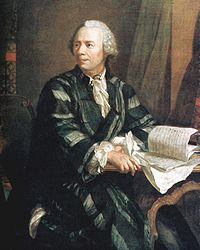
\includegraphics[width=0.2\textwidth]{euler}
\caption{Leonhard Paul \euler}
\end{figure}

\euler est considéré comme un éminent mathématicien du XVIIIe siècle et l'un des plus grands de tous les temps. 
Il est aussi l'un des plus prolifiques, et une déclaration attribuée à Pierre-Simon \bsc{Laplace} exprime l'influence d'\euler sur les mathématiques: \og Lisez \euler, lisez \euler, c'est notre maître à tous\fg{}.

Son \oe uvre est considérable. \euler intervint dans les trois domaines fondamentaux de la science de son époque: l'astronomie (orbites planétaires, trajectoires des comètes), les sciences physiques (champs magnétiques, hydrodynamique, optique, nature ondulatoire de la lumière,\dots) et les mathématiques, dans toutes ses branches, de l'arithmétique à la géométrie différentielle en passant par l'analyse numérique et fonctionnelle, le calcul des variations, les courbes et les surfaces algébriques, le calcul des probabilités et les premiers aspects de la théorie des graphes et de la topologie. 
Il introduisit également une grande partie de la terminologie et de la notation des mathématiques modernes, en particulier pour l'analyse mathématique, comme pour la notion d'une fonction mathématique. 
Il est également connu pour ses travaux en mécanique, en dynamique des fluides, en optique et en astronomie.


\euler est représenté sur la sixième série des billets suisses de 10~francs, sur de nombreux timbres postaux suisses, allemands et russes.

\begin{rmk}
Les éléments biographiques sont tirés de \url{http://fr.wikipedia.org/wiki/Euler}
\end{rmk}


 


\section{Quelques résultats mathématiques marquants}
Une des réussites d'\euler a été la démonstration du grand théorème de \textsc{Fermat} dans un cas particulier.

\begin{thm}[de \textsc{Fermat}, cas $n=3$]\label{theoreme.I}
L'équation $x^3 + y^3 + z^3 = 0$ n'admet aucune solutions entières lorsque $xyz \neq 0$.
\end{thm}

Le théorème~\ref{theoreme.I} est un résultat de théorie des nombres, mais \euler a touché à d'autres domaines. Citons par exemple ce résultat de topologie.

\begin{thm}
Il n'est pas possible de traverser tous les ponts de Könisberg en ne passant qu'une seule fois sur chaque pont.
\end{thm}

\begin{proof}
Il suffit d'associer un graphe à la ville comme dans la figure~\ref{fig:Königsberg} et de supposer que la promenade recherchée existe. 
On peut alors, à partir de la promenade, ordonner les sept arêtes du graphe de façon à ce que deux arêtes consécutives par rapport à notre ordre soient adjacentes dans le graphe (en considérant que la dernière et la première arête sont consécutives, puisqu'il y a retour au point de départ). 
Ainsi tout sommet du graphe est-il nécessairement incident à un nombre pair d'arêtes (puisque s'il est incident à une arête il est aussi incident à l'arête précédente ou qui lui succède dans l'ordre). 
Mais le graphe a des sommets qui sont incidents à trois arêtes, d'où l'impossibilité.\footnote{Source: \url{http://fr.wikipedia.org/wiki/Problème_des_sept_ponts_de_Königsberg}}
\end{proof}

\begin{rmk}
Notons que même si on renonce à exiger le retour au point de départ, une promenade traversant une et une seule fois chaque pont n'existe pas. Elle existerait si au plus deux sommets du graphe, correspondant aux points à choisir respectivement comme départ et arrivée, étaient incidents à un nombre impair d'arêtes. Or les sommets du graphe des ponts de Königsberg sont tous les quatre dans ce cas, on est donc loin du compte. Il suffirait cependant de supprimer ou de rajouter un pont quelconque pour que le graphe modifié permette des promenades tous ponts sans retour (seuls deux sommets restant d'incidence impaire). Et ce sont au moins deux ponts, bien choisis, qu'il faudrait ajouter ou retirer pour permettre la promenade avec retour initialement visée.
\end{rmk}

\begin{figure}
\centering
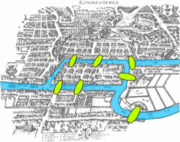
\includegraphics[width=0.25\textwidth]{l}%
\hfill
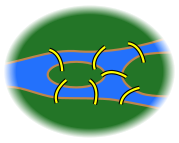
\includegraphics[width=0.25\textwidth]{c}%
\hfill
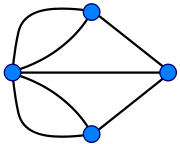
\includegraphics[width=0.25\textwidth]{r}
%
\caption{La ville de Königsberg (aujourd'hui Kaliningrad) est construite autour de deux îles situées sur le Pregel et reliées entre elles par un pont. Six autres ponts relient les rives de la rivière à l'une ou l'autre des deux îles. Le problème consiste à déterminer s'il existe ou non une promenade dans les rues de Königsberg permettant, à partir d'un point de départ au choix, de passer une et une seule fois par chaque pont, et de revenir à son point de départ, étant entendu qu'on ne peut traverser le Pregel qu'en passant sur les ponts.}
\label{fig:Königsberg}
\end{figure}



\subsection{Quelques formules mathématiques célèbres}

Voici quelques formules célèbres dues à Euler:
\begin{align}
e^{i\pi} &= -1,
\\
\pi &= \sqrt{ 6 \sum_{n=1}^\infty \frac{1}{n^2} },
\\
\lim_{n \to \infty} \left( \sum_{i=1}^n \frac{1}{i} \right) &= \ln(n) + \gamma + O\left(\frac{1}{n}\right),
\\
S-A+F &= 2. \label{eq:saf}
\end{align}
La formule~\eqref{eq:saf} lie le nombre de sommets $S$, d'arêtes $A$ et de faces $F$ d'un polyèdre convexe.



\subsection{Les méthodes d'\euler pour l'approximation des équations différentielles ordinaires}

\begin{defi}
Une équation différentielle (EDO) est une équation, dont l'inconnue est une fonction $y$, exprimée sous la forme d'une relation $F(y(t),y'(t),y''(t),\dots,y^{(n)}(t))=g(t)$, dans laquelle cohabitent à la fois $y=y(t)$ et ses dérivées $y'$, $y''$, \dots ($n$ est appelé l'ordre de l'équation). Si la fonction $g$, appelée \og second membre\fg{} de l'équation, est nulle, on dit que l'équation en question est homogène. 
\end{defi}

Nous pouvons nous limiter aux équations différentielles du premier ordre, car une équation d'ordre $n>1$ peut toujours se ramener à un système de $n$ équations d'ordre $1$. Une équation différentielle ordinaire admet généralement une infinité de solutions. Pour en sélectionner une, on doit imposer une condition supplémentaire qui correspond à la valeur prise par la solution en un point de l'intervalle d'intégration. On considérera par conséquent des problèmes, dits de \textsc{Cauchy}, ainsi défini:
\begin{defi}[Problème de \textsc{Cauchy}]
Soit $f \colon I \times \R \to \R$ une fonction donnée et $y'$ la dérivée de $y$ par rapport à $t$. On appelle \emph{problème de \textsc{Cauchy}} le problème
\begin{center}
trouver $y \colon I\subset \R \to \R$ tel que
\begin{equation}\label{eq:cauchy}
\begin{cases}
y'(t) = f(t,y(t)), &\forall t \in I,\\
y(t_0) = y_0,
\end{cases}
\end{equation}
\end{center}
avec $t_0$ un point de $I$ et $y_0$ une valeur appelée donnée initiale.
\end{defi}

\begin{thm}[Théorème de \textsc{Cauchy}-\textsc{Lipschitz}]
Soit un problème de \textsc{Cauchy}. Si la fonction $f(t,y)$ est
\begin{enumerate}
\item continue par rapport à ses deux variables;
\item lipschitzienne par rapport à sa deuxième variable, c'est-à-dire qu'il existe une constante positive $L$ (appelée constante de Lipschitz) telle que
\[
|f(t, y_1 ) - f(t, y_2 )| \le L|y_1 - y_2 |,\qquad \forall t \in I,\quad \forall y_1,y_2 \in \R,
\]
\end{enumerate}
alors la solution $y = y(t)$ du problème de \textsc{Cauchy} existe, est unique et appartient à $\mathcal{C}^1(I)$.
\end{thm}


Considérons le problème de \textsc{Cauchy}~\eqref{eq:cauchy} et supposons que l'on ait montré l'existence d'une solution $y$. Le principe des méthodes d'\euler est de subdiviser l'intervalle $I=[t_0,T]$, avec $T<+\infty$, en $N_h$ intervalles de longueur $h=(T-t_0)/N_h=t_{n+1}-t_n$; $h$ est appelé le pas de discrétisation. 
\begin{center}
\begin{tikzpicture}
\draw[blue] (0,0) -- (10,0);
\foreach \x in {0,1,...,10} \draw (\x,1pt)--(\x,-1pt) node[below]{$t_{\x}$};
\end{tikzpicture} 
\end{center}
Alors, pour chaque nœud $t_n=t_0 + nh$ on cherche la valeur inconnue $u_n$ qui approche $y(t_n)$. L'ensemble des valeurs $\{u_0 = y_0, u_1,\dots , u_{N_h} \}$ représente la solution numérique. Les schémas qu'on va construire permettent de calculer $u_{n+1}$ à partir de $u_n$ et il est donc possible de calculer successivement $u_1$, $u_2$,\dots en partant de $u_0$. Si nous intégrons l'EDO $y'(t)=f(t,y(t))$ entre $t_n$ et $t_{n+1}$ nous obtenons
\[
y(t_{n+1})-y(t_n)=\int_{t_n}^{t_{n+1}} f(t,y(t))dt.
\]
Soit $u_n$ une approximation de $y(t_n)$ et $u_{n+1}$ une approximation de $y(t_{n+1})$. On peut construire différentes schémas selon la formule de quadrature utilisée pour approcher le membre de droite. 
\begin{itemize}
\item Si on utilise la formule de quadrature du rectangle à gauche, \ie
\[
\int_{t_n}^{t_{n+1}} f(t,y(t))dt\approx h f(t_n,y(t_n))
\]
on obtient le \textbf{\emph{schéma d'\euler progressif}}
\[
\begin{cases}
u_0=y(y_0)=y_0,\\
u_{n+1}=u_n+h f(t_n,u(t_n))& n=0,1,2,\dots
\end{cases}
\]
Il s'agit d'un schéma explicite car il permet d'expliciter $u_{n+1}$ en fonction de $u_n$.
\item Si on utilise la formule de quadrature du rectangle à droite, \ie
\[
\int_{t_n}^{t_{n+1}} f(t,y(t))dt\approx h f(t_{n+1},y(t_{n+1}))
\]
on obtient le \textbf{\emph{schéma d'\euler rétrograde}}
\[
\begin{cases}
u_0=y(y_0)=y_0,\\
u_{n+1}-h f(t_{n+1},u_{n+1})=u_n& n=0,1,2,\dots
\end{cases}
\]
Il s'agit d'un schéma implicite car il ne permet pas d'expliciter directement $u_{n+1}$ en fonction de $u_n$ lorsque la fonction $f$ n'est pas triviale. \end{itemize}

\begin{exe}
On considère le problème de \textsc{Cauchy}
\[
\begin{cases}
y'(t)=-y(t),\\
y(0)=1,
\end{cases}
\]
sur l'intervalle $[0;3]$. La solution exacte est $y(t)=e^{-t}$ donc $y(3)=e^{-3}\simeq0.049787068$. Si on choisit $h=1/2$ on obtient 
\[
\begin{array}{|c|l|c|c|}
\hline
n&t_n&u_n=\frac{1}{2^n} \text{ (schéma progressif)}&u_n=\left(\frac{2}{3}\right)^n \text{ (schéma rétrograde)}\\
\hline
0&0&1&1\\
1&0.5&1/2&2/3\\
2&1&1/4&4/9\\
3&1.5&1/8&8/27\\
4&2&1/16&16/81\\
5&2.5&1/32&32/243\\
6&3&1/64\simeq0.015625&64/729\simeq0.087791495\\
\hline
\end{array}
\]
\end{exe}


\end{document}
